\section{Results}

We finally implemented our RSP heuristic algorithm on a simple aircraft design problem. 
In this problem, we conduct an aerostructural optimization of a wing and fuselage given a payload and a range requirement. 

% We implemented the RSP formulation ideas above on a simple aircraft design problem, with 12 uncertain variables,
% and a single signomial constraint. . A short overview of the model follows.

\subsection{Optimization Results}

The problem is optimized for different sizes of box and elliptical uncertainty sets
by varying the parameter $\Gamma$ as defined in Appendix \ref{LP_to_GP}.
The design variables are then fixed for each solution so that the design can be simulated for
1000 different realizations of the uncertain parameters in Table~\ref{tab:uncertainties}
to examine average design performance.\\

\begin{figure}[ht]
    \centering
    \captionsetup{justification=centering, font=small}
    \begin{subfigure}{0.49\textwidth}
        \centering
        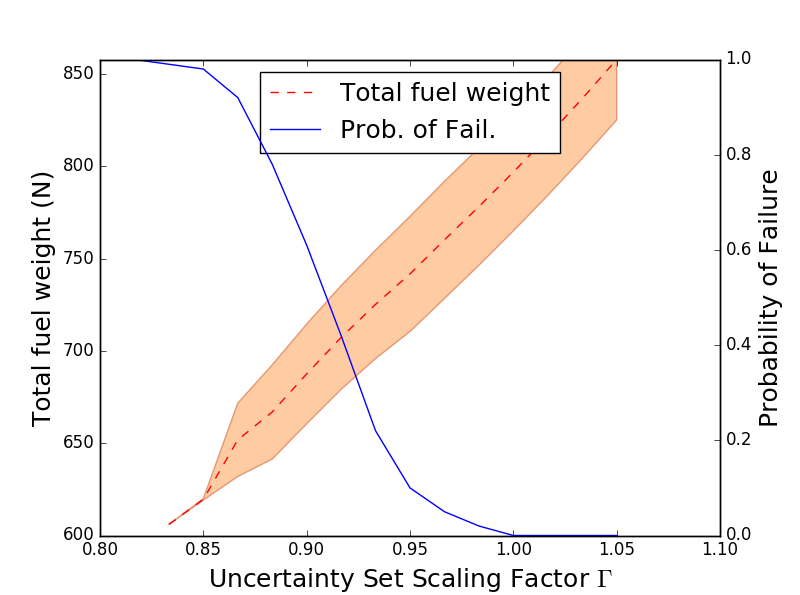
\includegraphics[height=2.3in]{signomial_simple_flight/box_best_pairs.png}
        % \caption{Box Uncertainty Set Objective Value}
    \end{subfigure}%
    ~ 
    \begin{subfigure}{0.49\textwidth}
        \centering
        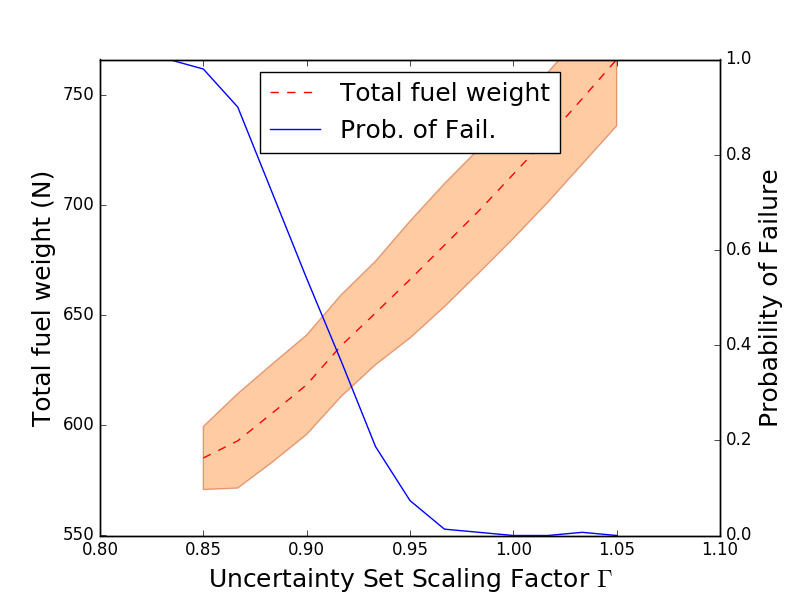
\includegraphics[height=2.3in]{signomial_simple_flight/ell_best_pairs.png}
        % \caption{Box Uncertainty Set Probability of Failure}
    \end{subfigure}
    \caption{Performance of the optimal robust signomial simple aircraft, using the Best Pairs formulation, as a function of $\Gamma$ for different uncertainty sets.}
    \label{signomial_var_gamma}
\end{figure}

We can see from Figure \ref{signomial_var_gamma} that probability of failure goes to zero as $\Gamma$ increases. 
Obviously, it is worth using elliptical uncertainty sets for this aircraft design problem as the performance is significantly better than that of a box uncertainty set, despite the increase in complexity. 
Moreover, using margins would in the best case be as good as using a box uncertaintyset, and therefore will lead to an inferior performance.

Figure~\ref{compare_signomial} compares the different methodologies in terms of run times, number of constraints, and average performance. The Best Pairs and Linearized Perturbations achieves good performance, however the Best Pairs methodology needs the most number of constraints, while the Linearized perturbations requires the most setup and solve time. The Simple Conservative formulation is significantly faster than the other formulations and requires the least number of additional constraints.
\ \\
\ \\

\begin{figure}[ht]
    \centering
    \captionsetup{justification=centering, font=small}
    \begin{subfigure}{0.499\textwidth}
        \centering
        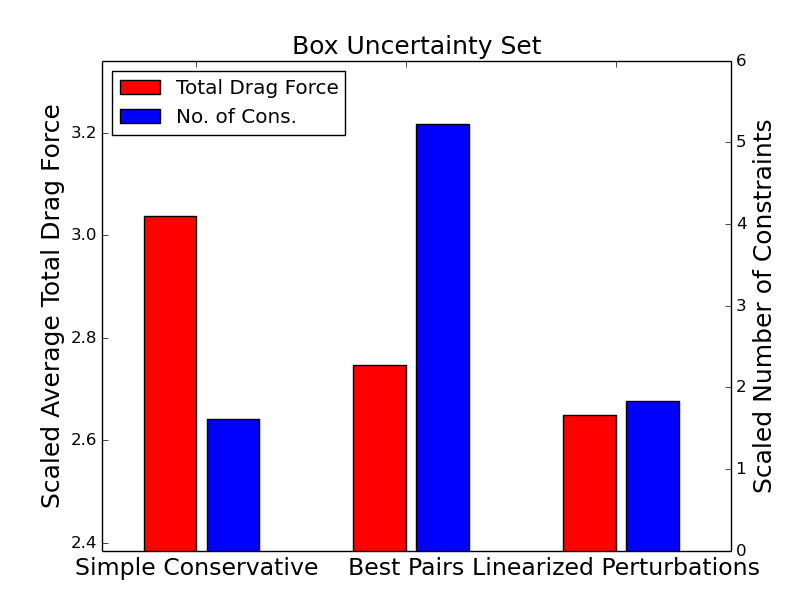
\includegraphics[height=2.3in]{signomial_simple_flight/box.png}
        % \caption{Box Uncertainty Set Objective Value}
    \end{subfigure}%
    ~ 
    \begin{subfigure}{0.49\textwidth}
        \centering
        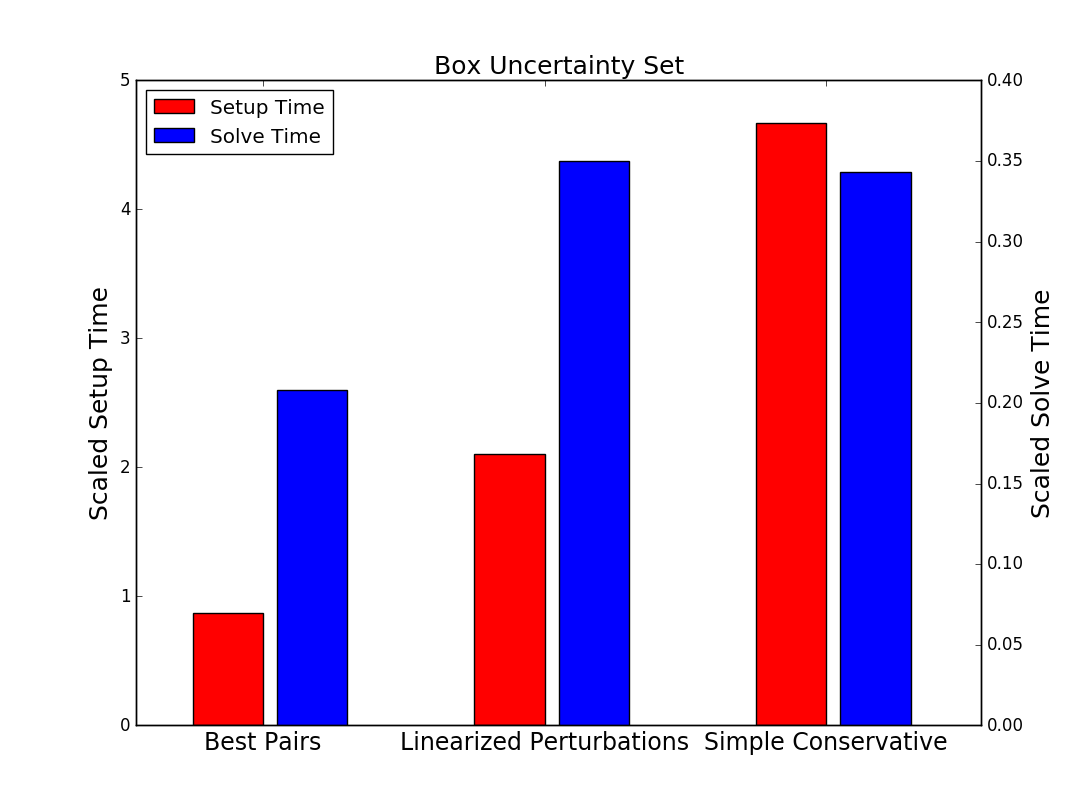
\includegraphics[height=2.3in]{signomial_simple_flight/box_times.png}
        % \caption{Box Uncertainty Set Probability of Failure}
    \end{subfigure}
    ~
    \begin{subfigure}{0.499\textwidth}
        \centering
        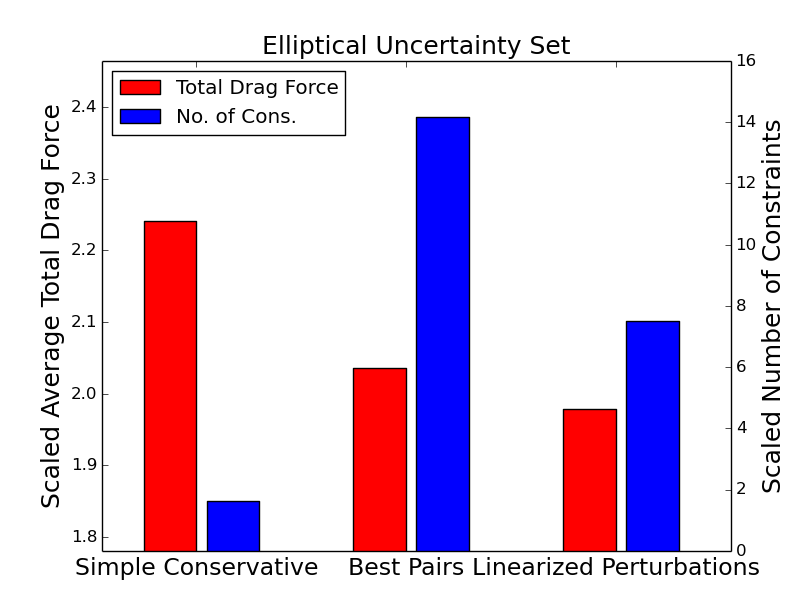
\includegraphics[height=2.3in]{signomial_simple_flight/ell.png}
        % \caption{Elliptical Uncertainty Set Objective Value}
    \end{subfigure}%
    ~ 
    \begin{subfigure}{0.49\textwidth}
        \centering
        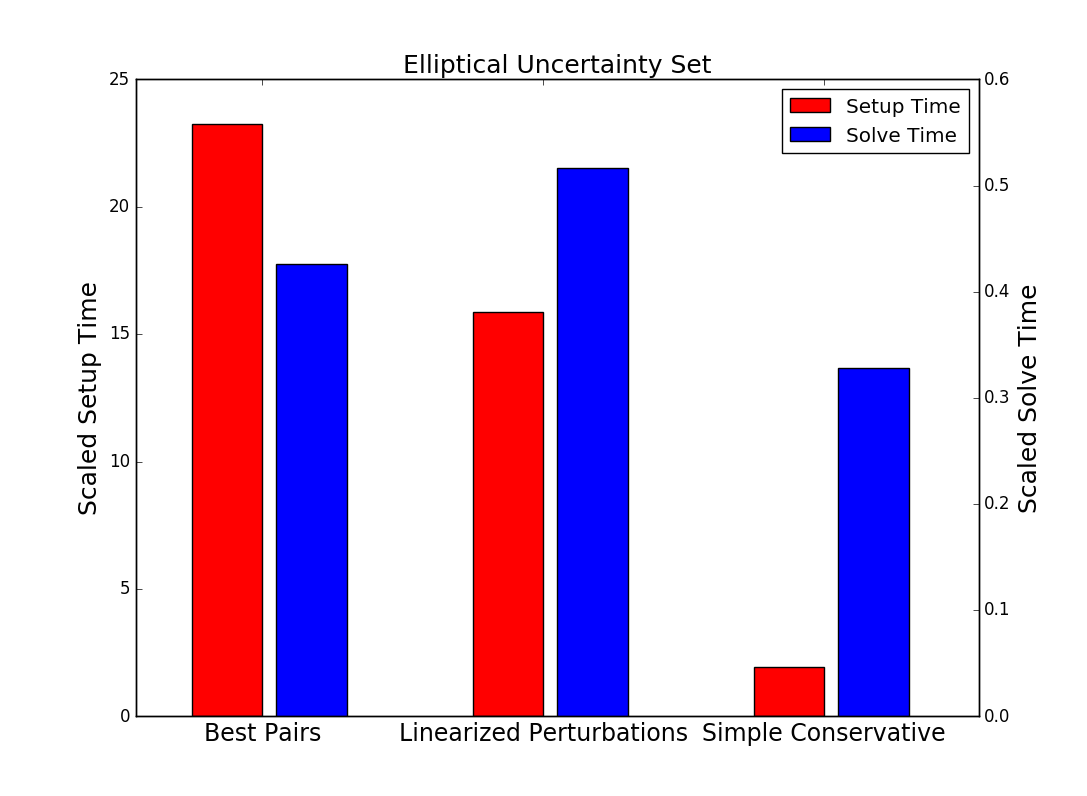
\includegraphics[height=2.3in]{signomial_simple_flight/ell_times.png}
        % \caption{Elliptical Uncertainty Set Probability of Failure}
    \end{subfigure}
    \caption{Robust signomial simple aircraft design results relative to the deterministic design problem.}
    \label{compare_signomial}
\end{figure}

\subsection{The Effect of Robustness}

\subsubsection{Multiobjective Spider Plots}

\begin{figure}
\begin{center}
\begin{tikzpicture}[scale=0.5]
\tkzKiviatDiagram{$\frac{W_f}{L/D}$,$D$,$W_f$}
%solve for {W_f}{L/D}
\tkzKiviatLine[thick,
color=red,
mark=ball,
ball color=red,
mark size=3pt,opacity=.2,
fill=red!20](154.4/25,414.2/75,5180/700)
%solve for D
\tkzKiviatLine[thick,
color=blue,
mark=ball,
mark size=3pt,
fill=blue!20,
opacity=.5](161.8/25,400/75,5129/700)
% solve for {W_f}
\tkzKiviatLine[thick,
color=yellow,
mark=ball,
mark size=3pt,
fill= yellow!20,
opacity=.5](190.2/25,463.4/75,4536/700)
\end{tikzpicture}
\end{center}
\caption[Deterministic Spider Plot]{Design optimization of the aircraft with no uncertainty for 3 different objective functions.
The red, blue and yellow correspond to $\frac{W_f}{L/D}$, $D$, $W_f$ and objectives respectively.}
% tkz-kiviat documentation here in FRENCH: http://mirror.jmu.edu/pub/CTAN/macros/latex/contrib/tkz/tkz-kiviat/doc/TKZdoc-kiviat-main.pdf
\label{fig:spiderplotnoUncert}
\end{figure}

%\textbf{TODO: update with 7-objective spider plots. First cite SP_tasopt, then show table and spider plots.
%Then show how robust results change the spider plots.}

\begin{table}
    \resizebox{\textwidth}{!}{
    \csvautobooktabularcenter{figures/objective_table.csv}
    }
\caption{Non-dimensionalized variations in objective values with respect to the aircraft optimized
for different objectives. Objective values were normalized by the total fuel solution.}
\end{table}

To further demonstrate the capabilities of robust SPs in aircraft design,
we performed the optimization of the aircraft with no uncertainty and ellipsoidal uncertainty ($\Gamma = 1$)
for two more objective functions, and plotted the results on spider plots.
Spider plots are useful because they allow engineers to find non-dominated solutions among the solutions
that lie on the Pareto frontier of potential objective functions. The objective functions chosen
for this analysis were fuel burn over lift-to-drag ratio ($\frac{W_f}{L/D}$), drag ($D$), and fuel burn ($W_f$).

In the spider plots in Figures \ref{fig:spiderplotnoUncert} and \ref{fig:spiderplotEllUncert},
none of the solutions are non-dominated for both the no uncertainty and ellipsoidal uncertainty cases.
In a GP, it is not possible that one of the solutions is non-dominated since the solutions are globally optimal.
But since there is no guarantee in optimality for SPs, it is possible to find non-dominated solutions if
the obtained solution is a local optimum.

In the case where there is no non-dominated solution such as this one,
we take the internal areas of the triangle formed by each optimization to be the figure of merit.
The smaller the area in the triangle, the higher the performance of the proposed solution.
In the no uncertainty case shown in Figure~\ref{fig:spiderplotnoUncert}, the red solution with the
objective of $\frac{W_f}{L/D}$ has the smallest internal area. In the ellipsoidal case shown in
Figure~\ref{fig:spiderplotEllUncert}, the blue solution with the objective of $D$ has the smallest internal area.

This is an interesting result, because the presence of an uncertainty set is
shown to affect the efficacy of different objective functions to obtain solutions
with the best overall performance. The differences between the objective functions
in the simple aircraft design problem are minute, because the different potential objectives
have a high degree of coupling. It is likely that, if the three objective functions didn't
have high degree of coupling, that the internal areas of the solution triangles may differ
more significantly.

%\begin{figure}
%\begin{center}
%\begin{tikzpicture}[scale=0.5]
%\tkzKiviatDiagram{$\frac{W_f}{L/D}$,$D$,$W_f$}
%%solve for {W_f}{L/D}
%\tkzKiviatLine[thick,
%color=red,
%mark=ball,
%ball color=red,
%mark size=3pt,opacity=.2,
%fill=red!20](568.6/100,1051/150,13500/1500)
%%solve for D
%\tkzKiviatLine[thick,
%color=blue,
%mark=ball,
%mark size=3pt,
%fill=blue!20,
%opacity=.5](587/100,1024/150,13100/1500)
%% solve for {W_f}
%\tkzKiviatLine[thick,
%color=yellow,
%mark=ball,
%mark size=3pt,
%fill= yellow!20,
%opacity=.5](687.9/100,1155/150,11900/1500)
%\end{tikzpicture}
%\end{center}
%\caption[Uncertain Spider Plot]{Design optimization of the aircraft with ellipsoidal uncertainty for 3 different objective functions.
%The red, blue and yellow correspond to $\frac{W_f}{L/D}$, $D$, $W_f$ and objectives respectively.}
%% tkz-kiviat documentation here in FRENCH: http://mirror.jmu.edu/pub/CTAN/macros/latex/contrib/tkz/tkz-kiviat/doc/TKZdoc-kiviat-main.pdf
%\label{fig:spiderplotEllUncert}
%\end{figure}

\subsection{Goal Programming}

However, this assumes that we have an understanding of exactly how much risk we are
willing to tolerate. This begs the question, could we have risk as the output of our
model? This would suggest the following formulation:

\begin{align*}
    \text{maximize} &~\Gamma \\
    \text{s.t.}     &~f_i(x,u) \leq 0, i = 1,\ldots,n \\
                    & \norm{u} \leq \Gamma \\
                    &~f_0(x) \leq (1+\delta)f_0^*,~\delta \geq 0 \tag{a}
    \label{eq:goalprogramming}
\end{align*}

where $f_0^*$ is the optimum of the original problem in Formulation~\ref{eq:normform}, $\delta$
is a fractional measure of the objective that we are willing to sacrifice for robustness, which
gives $(1+\delta)f_0^*$ as the upper bound on the objective value.

We can also expand this framework to perform multivariate goal programming,
by changing (a) in the formulation~\ref{eq:goalprogramming} to include all
objectives we are interested in.

\begin{align*}
    f_{0,j}(x) \leq (1+\delta_j) f^*_{0,j},~\delta_j \geq 0,~i = 1,\ldots, m
    \label{eq:multigoal}
\end{align*}

The benefit of goal programming is that it allows us to explore multidisciplinary tradeoffs without
having to enumerate the design space along each objective direction. Furthermore, in design it is not obvious whether
an objective should in fact be a constraint instead. For example, it's not clear that the design
of an aircraft is useful if it consumes

\subsubsection{Changes in flight envelope}
